\documentclass[conference]{IEEEtran}

\usepackage[T1]{fontenc}
\usepackage{booktabs}
\usepackage{amsmath}
\usepackage{xcolor}
\usepackage{graphicx}
\usepackage{tabularx}
\usepackage{tikz}
\usepackage{url}
\usepackage{hyperref}
\usepackage{microtype}
\usepackage{sc26repro}
\DisableLigatures{encoding = T1, family = pcr}
\usetikzlibrary{arrows.meta,positioning}

\hypersetup{colorlinks=true, linkcolor=blue!55!black,
  citecolor=blue!55!black, urlcolor=blue!55!black,
  pdftitle={Meganeura: Vulkan and Metal as a Performance-Portability Layer for GPU Training and Inference},
  pdfauthor={Dzmitry Malyshau},
  pdfsubject={SC26 P3HPC workshop paper},
  pdfkeywords={performance portability, Vulkan, Metal, GPU training, autotuning},
  pdfdisplaydoctitle=true}
% Long bibliography URLs must break inside two-column IEEE layout.
\expandafter\def\expandafter\UrlBreaks\expandafter{\UrlBreaks\do\-\do\_\do\.}

\newcommand{\system}{Meganeura}
\newcommand{\inferena}{Inferena}
\newcommand{\code}[1]{\texttt{#1}}

\title{Meganeura: Vulkan and Metal as a Performance-Portability Layer\\
for GPU Training and Inference}

\author{\IEEEauthorblockN{Dzmitry Malyshau}
\IEEEauthorblockA{Independent Researcher\\
kvark@fastmail.com \quad ORCID: 0009-0005-6410-4276}}

\begin{document}
\maketitle

\begin{abstract}
Graphics application programming interfaces (APIs) already reach most
consumer graphics processing units (GPUs). Can they also support a useful
machine-learning runtime? Meganeura is a compact native compiler and runtime
that lowers tensor graphs and automatic differentiation to Vulkan and Metal.
Its compilation step retains graph alternatives in an e-graph and measures
their kernel implementations.
We compare five workloads with compiled PyTorch at one source revision,
using CUDA, HIP, and XPU graph replay where available.
The six-platform benchmark qualifies all 180 inference process pairs and
174 training pairs. Across qualified strict 32-bit floating-point
comparisons, median inference and training times are $1.27\times$ and
$1.92\times$ PyTorch's. PyTorch Whisper training fails repeatability on
RX~7900~XT; separate eager checks validate Meganeura without replacing the
failed timings. Three further integrated GPUs pass Vulkan qualification
without a qualified PyTorch GPU comparison. Larger models extend the study
to 1.7 billion parameters on H100. Their inference gap grows with size,
despite a narrowing strict training gap. Graphics APIs offer useful
deployment reach, but kernel efficiency and search cost still need work.
\end{abstract}

\begin{IEEEkeywords}
performance portability, GPU, Vulkan, Metal, machine learning systems,
training, correctness validation
\end{IEEEkeywords}

\section{Introduction}

In high-performance computing (HPC), portability layers such as Kokkos,
RAJA, and SYCL let one program target heterogeneous hardware
\cite{edwards2014kokkos,beckingsale2019raja,khronos2020sycl}.
Graphics APIs offer another route for machine learning
(ML): Vulkan exposes cross-vendor graphics and compute, while Metal
serves Apple platforms \cite{khronos2026vulkan,apple2026metal}.
An application already using these APIs can share its resources and
execution queue with a tensor runtime. This is especially useful in games
and interactive applications: ML need not introduce a second GPU stack.
We measure what this choice gains in hardware coverage and costs in speed.

\system{} is a small native compiler and runtime. It lowers a typed tensor
graph, and the training graph that automatic differentiation builds from
it, to specialized compute kernels. Blade is the Vulkan and Metal layer
\cite{malyshau2026barriers}. Construction, differentiation, checkpoints,
and the runtime interface are shared across devices, so a deployed
application does not need Python or a vendor machine-learning runtime.
Training and inference use the same compiler. Compilation can time
alternative graphs and kernels before it commits to a plan. That search
is off unless the caller requests it. Every native session in the primary
cohort requests it.

The evaluation compares \system{} with PyTorch
\cite{paszke2019pytorch} at one source commit across CUDA, ROCm, XPU, MPS,
and CPU-oracle wheels. Every timed reference in the primary cohort uses
default compilation. CUDA, HIP, and
XPU execute explicitly captured, numerically qualified whole-phase graphs;
MPS has no equivalent public replay interface. Native empirical selection
is always enabled, independently of the reference's compiler mode.
We report preparation time separately from steady-state execution.

Performance, portability, and productivity (P3) ask different questions.
How fast does the workload run? Can it run on the device at all? How much
work does it take to develop and deploy it? We measure the first two and
some deployment costs. Three integrated GPUs qualify through Vulkan but
lack a qualified PyTorch GPU comparison; \system{} has no validated Vulkan path on the attempted
MI300X. Debugging and maintenance matter too, but binary size and
preparation time are not programmer-productivity scores
\cite{lin2024productivity}.

Our contributions are:
\begin{itemize}
  \item A numerically checked comparison on six GPU platforms and
        qualification on three more, including incomplete campaigns and
        the points where execution fails.
  \item Measurements of graph and kernel search inside compilation:
        which alternatives it visits, which it rejects, and what it costs.
  \item Host/GPU profiles and optimization experiments that explain
        several bottlenecks, plus same-revision measurements of models up
        to 1.7 billion parameters.
\end{itemize}

An arithmetic contract (Section~\ref{sec:contracts}) specifies permitted
numerical fast paths. Each device--workload--contract--policy comparison
is validated before its timings are admitted. Graphics-only qualification
remains visible without entering the GPU performance aggregate.
This includes datacenter hardware, but not production-scale large language
model (LLM) training, optimizer updates, distributed execution, or scientific
simulation workloads.
The companion technical report develops the compiler and system design
in greater detail \cite{malyshau2026meganeura}.

\section{The Layer Under Study}
\label{sec:system}

\begin{figure}[t]
\centering
\resizebox{0.91\columnwidth}{!}{%
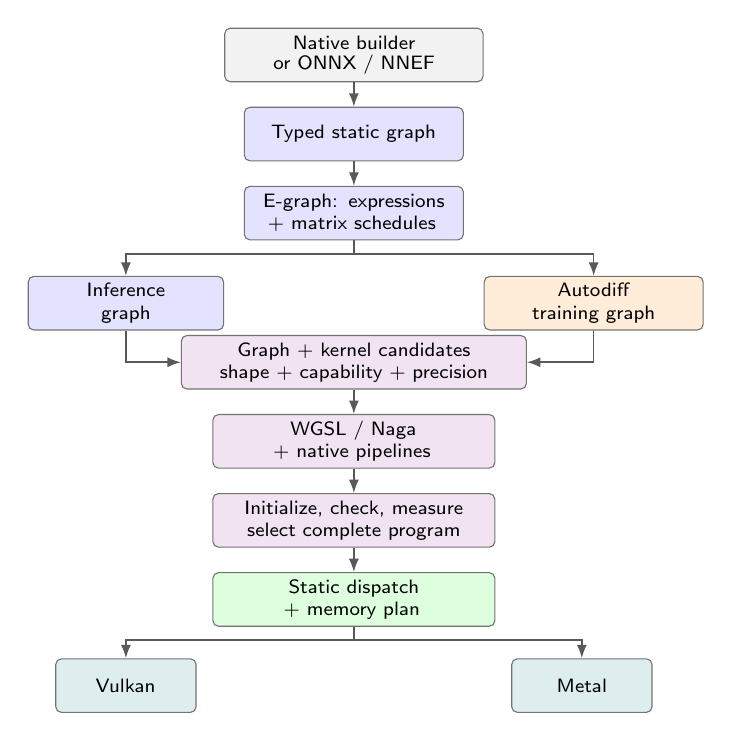
\begin{tikzpicture}[
  font=\sffamily\scriptsize,
  node distance=3.1mm,
  box/.style={draw=black!55, rounded corners=2pt, minimum height=6.8mm,
    align=center, inner xsep=4pt, inner ysep=2pt},
  source/.style={box, fill=gray!10},
  graph/.style={box, fill=blue!11},
  train/.style={box, fill=orange!15},
  compile/.style={box, fill=violet!11},
  runtime/.style={box, fill=green!13},
  backend/.style={box, fill=teal!13},
  arrow/.style={-{Latex[length=1.7mm]}, semithick, draw=black!65}
]
  \node[source, text width=30mm] (source)
    {Native builder\\[-0.1em]or ONNX / NNEF};
  \node[graph, text width=25mm, below=of source] (typed)
    {Typed static graph};
  \node[graph, text width=25mm, below=of typed] (rewrite)
    {E-graph: expressions\\+ matrix schedules};
  \node[graph, text width=22mm, below left=4.5mm and 2.5mm of rewrite] (infer)
    {Inference\\graph};
  \node[train, text width=25mm, below right=4.5mm and 2.5mm of rewrite] (training)
    {Autodiff\\training graph};
  \node[compile, text width=41mm, below=12mm of rewrite] (specialize)
    {Graph + kernel candidates\\shape + capability + precision};
  \node[compile, text width=33mm, below=of specialize] (naga)
    {WGSL / Naga\\+ native pipelines};
  \node[compile, text width=33mm, below=of naga] (measure)
    {Initialize, check, measure\\select complete program};
  \node[runtime, text width=33mm, below=of measure] (plan)
    {Static dispatch\\+ memory plan};
  \node[backend, text width=15mm, below left=4mm and 2mm of plan] (vulkan)
    {Vulkan};
  \node[backend, text width=15mm, below right=4mm and 2mm of plan] (metal)
    {Metal};

  \draw[arrow] (source) -- (typed);
  \draw[arrow] (typed) -- (rewrite);
  \draw[arrow] (rewrite.south) -- ++(0,-1.7mm) -| (infer.north);
  \draw[arrow] (rewrite.south) -- ++(0,-1.7mm) -| (training.north);
  \draw[arrow] (infer.south) |- (specialize.west);
  \draw[arrow] (training.south) |- (specialize.east);
  \draw[arrow] (specialize) -- (naga);
  \draw[arrow] (naga) -- (measure);
  \draw[arrow] (measure) -- (plan);
  \draw[arrow] (plan.south) -- ++(0,-1.7mm) -| (vulkan.north);
  \draw[arrow] (plan.south) -- ++(0,-1.7mm) -| (metal.north);
\end{tikzpicture}%
}
\caption{The shared compilation path. Each forward-graph candidate can
produce its own differentiated training graph. Explicit matrix schedules
are preserved; remaining kernel choices are tuned before programs compete.}
\label{fig:pipeline}
\end{figure}

\system{} executes a typed static tensor graph (Figure~\ref{fig:pipeline}).
Native builders and importers for Open Neural Network Exchange (ONNX)
and Neural Network Exchange Format (NNEF) construct the graph.
Egglog retains equivalent expressions in an e-graph using bounded equality
saturation \cite{zhang2023egglog}. It adds alternatives to equivalence classes
instead of committing to the first profitable local rewrite. Search covers
small graphs or bounded regions of rewritable operators, including independent
projections. Larger cases fall back to verified repeated regions. Precision
domains and mutations are boundaries. Training adds reverse-mode
differentiation and, when requested by the application, a stochastic
gradient descent (SGD) or Adam update.
The benchmark measures forward, loss, and backward only.
The ordinary builder extracts one graph by estimated tensor traffic.
Measured construction keeps several forms until their implementations
have been timed. Both paths use the same e-graph rules, extractor, and lowering
code; there is no separate greedy optimizer. The cost counts logical tensor
bytes, not HBM transactions or latency: it omits caches, arithmetic,
occupancy and launch costs. It orders exploration, not the measured winner.

Matrix tile dimensions, K stages, counted or unrolled loops, and split-K
are implementation alternatives in the same e-graph. This covers
transposed products and packed projections. Lowering locks an extracted
schedule; an automatic alternative retains ordinary kernel probes, including
cooperative paths where legal. Derivative products inherit the forward
schedule subject to legality checks. Independent gradient schedules and
cooperative tile dimensions are not yet searched this way.
Some shape-based choices, including direct versus Winograd convolution,
remain outside this search.

Code generation uses a small set of reusable kernel families:
pointwise expressions, reductions, general matrix multiplication (GEMM), convolutions and
their derivatives, and tiled attention. Shape, device capabilities,
and precision policy determine legal implementations and workgroup
geometry. The generated WebGPU Shading Language (WGSL) is validated
by Naga \cite{w3c2026wgsl}; Blade lowers it for native Vulkan/Metal.
Sharing Naga with wgpu does not mean using the wgpu runtime or executing
in a browser.

The compiler fixes a dispatch sequence and lifetime-based buffer reuse.
Each step records and submits that plan without graph rediscovery or
per-step tensor allocation; host command recording and synchronization
remain. It does not replay a native CUDA Graph.
The reference therefore receives its native command-graph replay path,
rather than paying an avoidable per-step Python submission cost.

Measured construction initializes representative inputs and weights in
private sessions. It checks candidates against ordinary untuned execution,
tunes their legal kernels, then compares complete programs with fresh command
recording and submission. It keeps the current winner unless a candidate
passes the numerical checks and the paired timing noise guard.
Graph forms therefore compete after kernel search, rather than being
discarded before tuning begins. Finite budgets can leave that search
incomplete; retaining equivalent expressions does not guarantee faster code.

The measured policy allows sixteen graph/schedule forms and 64 programs
per session, with a shared 60-second search deadline. It interleaves graph
and physical-plan choices; private kernel probes use the remaining time
and at most 1\,GiB of scratch space, without a class-count cap.
The two active plans and state snapshots are bounded by 75\% of reported
available device memory; driver allocations and private scratch are additional.
Deadlines are soft around in-flight driver and validation work.
The search includes dispatch fusion and submission chunking as well as
kernel geometry. Paired whole-program comparisons require two warmup
pairs and 250\,ms, subject to that deadline. Bounded regions and repeated
blocks keep extraction manageable; the search does not cover every possible
partition of a large graph.

\section{Checking the Compiler and Its Kernels}
\label{sec:validation}

Agreement between two frameworks is useful evidence, but it does not tell
us which one is wrong when they disagree. Repeating a result is weaker
still: a deterministic indexing error repeats perfectly. We therefore
separate three checks in \system{}'s development suite. The measured
revision includes this suite and the fixes it prompted.\footnote{\href{https://github.com/kvark/meganeura/tree/0dbfcc0029bf98b33a03fc792e1f4e90ead17f23/src/reference}{Reference interpreter and checks at the measured revision}.}

First, a simple CPU interpreter evaluates graph operators in 64-bit
floating point, without sharing GPU lowering or shader code. Inputs are
rounded to their declared storage precision before evaluation. We compare
symbolic derivatives evaluated by this interpreter with central finite
differences. Nonuniform weighted losses exercise gradients other than
the special case of an all-ones upstream derivative; directional probes
check combinations of parameter elements. These tests exclude GPU execution
as a cause, although reference mistakes, finite-difference error, and
nondifferentiable inputs still need to be considered.

Second, operator-family sweeps compare every GPU output element and
parameter-gradient element with the interpreter. Shapes exercise tile
edges, reduction splits, and alternative lowerings. The default comparison
uses per-element magnitude scales, including sums of absolute products
for cancellation-prone reductions. This is a practical error model, not
a proved bound for every fused computation. Third, composed blocks and
seeded random graphs pass through differentiation, e-graph optimization,
dispatch fusion, and memory planning. Their outputs and gradients are
compared with the unoptimized reference, including gradients packed by
the optimizer. Nonparameter storage is initially filled with NaNs to expose
missing writes and invalid reuse.

These checks found dropped parameter gradients during fusion, loss
reductions that were not scalar, cancellation in normalization, and
vanishing GELU tails. They complement the broad state, checkpoint, loader,
and profiling tests rather than adding a separate executable for each bug.
An exhaustive operator match requires an explicit reference case or an
unsupported result when the IR grows; packed quantized formats remain
unsupported. Passing the tested graphs does not establish coverage of all
shapes, schedules, drivers, or devices.

The interpreter is a development tool, not a full-model oracle in the
timing loop. The benchmark instead applies fixed repeatability and
cross-engine gates (Section~\ref{sec:gates}). The collector
treats a failed reference as an outcome: qualified inference remains
available if training fails, and the failed compiled phase retains no
accepted timing. One fresh eager, uncaptured PyTorch process with math
attention checks the same weights, inputs, device, and arithmetic contract.
It must pass the same repeatability gates before serving as a separate
correctness reference. It never supplies replacement compiled timings.
Unexplained execution faults stop collection; classified numerical failures
do not prevent the remaining planned conditions from running. Failed and
unreached phases remain in the coverage counts, and incomplete replicate
groups stay out of aggregate speed comparisons.

\section{Methodology}
\label{sec:method}

\inferena{}, the open-source cross-framework harness, constructs matched
workloads, alternates engine order, synchronizes timing boundaries,
and records raw samples, outputs, gradient norms, revisions, and
environment metadata.\footnote{\href{https://github.com/kvark/inferena/tree/7b8fcb72e55410d8e33bbe948f89be50c691fcf7}{Inferena source, revision \code{7b8fcb72}}.}
It supplies kernels to neither engine.

\subsection{Revisions and reference conditions}
\label{sec:reference-policy}

The campaigns use \inferena{} \code{7b8fcb72} and
\system{} \code{0dbfcc00}, with Blade \code{fbb4f28}.
All wheels report PyTorch 2.13.0 at source
commit \code{cf30153}, with Python 3.13.13. NVIDIA uses
\code{+cu130}, AMD \code{+rocm7.2}, Arc \code{+xpu}, Apple the MPS
wheel. RPL-U uses a CPU wheel for qualification; the two Radeon iGPU runs use
the ROCm wheel with the CPU backend explicitly selected. None supplies
a CPU-versus-GPU timing comparison.
Checkpoint revisions and hashes are recorded in the manifests.
Driver, host, and backend-library differences remain part of the platform;
a common PyTorch revision does not make those implementations identical.

Arithmetic and preparation are separate axes. Both arithmetic contracts
pair tuned Meganeura with default-compiled PyTorch.
We choose this preparation policy because max-autotune was costly and
unreliable during bring-up: lengthy compilation on H100, failed convolution
searches on Radeon, and stalled qualification on Arc
(Section~\ref{sec:availability}). These observations motivate the policy;
no earlier timing enters the comparison.
Default compilation gives every backend the same practical reference policy.

PyTorch's \code{max-autotune}, GEMM/pointwise search and coordinate-descent
options are disabled; default compiler and vendor-library heuristics still
apply \cite{pytorch2026compile}. A supervisor enforces a 120-second
compilation deadline covering the first forward, backward, and minimal-shape
specializations, terminating compiler descendants on failure.
Model loading, graph capture, and research validation are outside that deadline.
Meganeura uses the per-session search ceiling above. The limits have
different scopes: this is not an equal-budget contest or a comparison
with the best PyTorch result obtainable after hours of search.

CUDA and ROCm use \path{torch.cuda.CUDAGraph}; ROCm maps that interface
to HIP graphs. Intel uses \path{torch.xpu.XPUGraph}
\cite{pytorch2026hip,pytorch2026xpugraph}.
Inductor's internal \code{triton.cudagraphs} mechanism is disabled so the
explicit capture is the sole replay owner. XPU uses the public math
scaled-dot-product-attention (SDPA) backend to accommodate graph capture;
the setting and a qualified embedding-backward workaround are recorded
(Section~\ref{sec:availability}). Other backends retain automatic SDPA
selection in the timed cohort. Failed ROCm Whisper training gets a separate
eager/math diagnostic, not a change to the timed policy.
MPS also compiles all requested
phases. MPS's Inductor path is exercised \cite{pytorch2026mpssource}, but
the pinned MPS API offers no equivalent public whole-phase replay interface.
MPSGraph execution is not CUDA Graph capture. No failed compiled or
captured condition may silently substitute eager or CPU execution.

\subsection{Workloads and timing}

The five principal workloads are SmolLM2-135M (decoder-only transformer)
\cite{benallal2025smollm2},
the SmolVLA action expert (99.85M parameters)
\cite{shukor2025smolvla}, a scaled Stable Diffusion 1.x U-Net
(10.93M, not checkpoint-compatible with SD~1.5)
\cite{rombach2022ldm}, ResNet-50 at batch four
\cite{he2016resnet}, and the Whisper-tiny encoder (8.21M)
\cite{radford2022whisper}. Both runners use the same shapes,
deterministic inputs, scalar objective, and canonical parameter names.
SmolLM2 uses pinned public checkpoints. The other workloads use matched,
deterministic uniform parameters (\path{name-index-uniform-v1}), not trained
task models. Section~\ref{sec:scaling} adds SmolLM2-360M on three platforms
and SmolLM2-1.7B on H100 at the same source and protocol revisions.

Three phases are timed: full no-gradient forward, minimal-shape forward,
and forward--loss--backward (F+L+B), without an optimizer update.
SmolLM2 uses batch one, 128-token prefill and one stateless token.
There is no key/value cache; the latter is not an autoregressive serving
benchmark. Whisper's full and minimal shapes coincide.
Each phase warms for at least five calls and two seconds, followed by
20 synchronized host-wall samples.
Input loading and output/gradient readback occur outside the timing
interval. Buffers are initialized before execution; the retained planner
memory counts do not prove physical residency of every binding.

Each condition runs in three fresh process pairs, with alternating
engine order and rotated condition order. We report the median of the
three within-process medians, and retain their range and all samples.
Twenty calls in one process are not twenty independent replicates.
Each phase needs three qualified pairs to enter a timing aggregate.
A failed backward pass does not discard qualified inference, and an eager
diagnostic never fills a missing compiled result. The conditional
portability score uses a fixed subset with all phases complete.
No older result fills a missing run.
Unreached conditions are unmeasured, not framework failures.

\subsection{Arithmetic contracts}
\label{sec:contracts}

Strict f32 disables TensorFloat-32 (TF32) in PyTorch and reduced-input
cooperative-matrix paths in \system{}. Tensor storage,
accumulation, and outputs remain f32.
Qualified f32-input/f32-accumulate cooperative tiles are allowed: this
contract preserves arithmetic width, not reduction order. Apple M3 exposes
such tiles and records strict cooperative dispatches in all five workloads;
the measured Vulkan devices expose none through this stack.
The accelerated contract permits PyTorch's TF32 paths and
\system{}'s supported cooperative implementations, including
f16-input/f32-accumulate forward matrix, convolution, and attention work.
Derivative regions retain the full-precision policy.
The permissions are not identical numerical formats, and a device may
expose no implementation that engages them.
No quantization or persistent f16 tensor storage is enabled.

\subsection{Independent numerical gates}
\label{sec:gates}

Cross-engine forward validation checks shape, relative L2 error below
1\% over 256 evenly spaced output samples, and relative scalar-loss
error below 1\%. Backward validation additionally checks canonical
parameter sets, total-gradient-norm error, and relative L2 error of the
per-parameter norm vector. Packed native gradients are restored to the
original checkpoint coordinates before computing norms.
Strict runs require both gradient errors below 5\%.
The frozen accelerated replication rule requires each error below 10\%
and the median of three process errors below 5\%, accommodating permitted
nondeterminism without accepting an unbounded outlier.
All 198 complete GPU pairs, including the larger models, and 30 CPU-oracle
qualification pairs individually stay below 5\%. The largest
parameter-norm-vector error is 0.296\%, sampled-output error 0.241\%, and
scalar-loss error 0.0140\%. The six partial pairs retain valid inference;
their separate eager diagnostics also validate native gradients.
The offline audit recomputes these gates and the three-process gradient
rule for every complete timing group.
Norm checks can miss sign or elementwise errors, and sampled outputs
can miss localized errors.

PyTorch first checks full-element repeatability, including on MPS and CPU.
CUDA, HIP, and XPU then check two consecutive graph replays against the
first uncaptured result. Preparation, warmup, capture, and execution on
these backends share one dedicated stream.
Every participating output and gradient element is checked.
Accelerated training uses eight uncaptured repeats; other phases use two.
Each output and loss tensor must satisfy both a maximum-error and a
root-mean-square (RMS) error bound: $10^{-6}+10^{-4}r$, where $r$ is the
corresponding reference maximum or RMS. This avoids a near-zero-sensitive pointwise
relative test without fitting tolerances to observed repeats.
Strict gradients use those bounds per parameter and over the whole gradient;
accelerated gradients use whole-gradient bounds with coefficient $10^{-2}$.
Ordinary repeatability and replay errors are recorded separately against
the first uncaptured result.
Classified numerical failures preserve completed phases and allow the next
condition to run; unclassified execution faults stop the campaign.
No eager timing replaces a failed graph run.
The retained reports establish that this qualification ran, but do not
contain all tensor elements for independent offline revalidation.

\subsection{Machines and coverage}

\begin{table*}[t]
\caption{Recorded environments and qualified process pairs per phase,
out of 30 planned on each platform.}
\label{tab:devices}
\centering
\small
\setlength{\tabcolsep}{5pt}
\begin{tabular}{llllrl}
\toprule
Device & PyTorch path & Graphics driver & Explicit replay & Pairs & Campaign \\
\midrule
RTX 5070 & CUDA/compiled & 595.91.07 & CUDA Graph & 30/30 & complete \\
H100 & CUDA/compiled & 580.126.09 & CUDA Graph & 30/30 & complete \\
RTX 3050 (Windows) & CUDA/compiled & 591.86 & CUDA Graph & 30/30 & complete \\
RX 7900 XT & ROCM/compiled & Mesa 26.0.3 & HIP graph & 30/30 & complete \\
Radeon 780M & ROCM/compiled & Mesa 25.2.8 & HIP graph & 25/30 & incomplete \\
Arc B570 & XPU/compiled & Mesa 26.0.3 & XPU graph & 30/30 & complete \\
Apple M3 & MPS/compiled & Metal & no public replay & 30/30 & complete \\
\bottomrule
\end{tabular}

\end{table*}

Table~\ref{tab:devices} lists six GPU-reference configurations.
RTX~5070, H100, Windows RTX~3050, Arc~B570, and Apple~M3 each complete
all 30 pairs. RX~7900~XT completes 24 full pairs and six inference-only
pairs: Whisper training fails repeatability in every process under both
contracts. Minimal-shape timing follows training and is not reached in
those processes, even though Whisper's two inference shapes coincide.
The main matrix therefore has 180 qualified inference pairs and 174
qualified pairs in each other phase. All 24 larger-model pairs on
RTX~5070, RX~7900~XT, and H100 pass.
RTX~3050 runs natively on Windows with driver 591.86;
the other Vulkan campaigns run on Linux, and M3 uses macOS.
RTX~5070 and B570 share the same host and are measured sequentially,
not concurrently. B570 uses a secondary PCIe~3.0 $\times$1 link;
the study does not normalize interconnect bandwidth across platforms.
Two additional campaigns stop at their first strict condition: 135M on
Radeon~780M and 360M on B570. Both fail in PyTorch; neither supplies a
paired timing. The remaining 29 and five pairs are unreached, not failed.
Radeon~780M, Ryzen~9600X's integrated Radeon, and Intel RPL-U each pass
all ten Vulkan qualification conditions against eager CPU PyTorch
(Table~\ref{tab:qualification}). These use one process per condition;
their timings do not enter any GPU comparison.

\section{Results}
\label{sec:results}

\begin{table*}[t]
\caption{Meganeura/PyTorch time ratios: native tuning versus default compilation.
$n$ counts processes with qualified inference (strict/accelerated).
Where PyTorch fails or does not reach a phase, M gives the independently
qualified native time in milliseconds, not a ratio.}
\label{tab:performance}
\centering
\small
\setlength{\tabcolsep}{4pt}
\begin{tabular}{llrrrrrr}
\toprule
Device & Workload & \multicolumn{3}{c}{Strict} & \multicolumn{3}{c}{Accelerated} \\ \cmidrule(lr){3-5}\cmidrule(lr){6-8} & & Inf. & Min. & F+L+B & Inf. & Min. & F+L+B \\
\midrule
RTX 5070 & SmolLM2-135M & 2.09 & 1.58 & 3.07 & 3.75 & 1.57 & 4.74 \\
 & SmolVLA & 2.03 & 1.66 & 2.47 & 3.57 & 1.62 & 3.43 \\
 & StableDiffusion & 1.40 & 1.39 & 3.05 & 2.06 & 1.96 & 5.05 \\
 & ResNet-50 & \textbf{1.00} & 1.24 & 3.02 & 2.80 & 3.48 & 6.05 \\
 & Whisper-tiny & 2.73 & 2.72 & 2.89 & 1.87 & 1.88 & 2.97 \\
H100 & SmolLM2-135M & 3.99 & 1.44 & 5.28 & 5.19 & 1.44 & 7.30 \\
 & SmolVLA & 2.14 & 1.02 & 3.23 & 4.68 & 1.58 & 4.78 \\
 & StableDiffusion & 1.83 & 1.73 & 3.35 & 3.35 & 3.28 & 5.41 \\
 & ResNet-50 & 2.10 & 2.48 & 6.40 & 8.51 & 9.75 & 20.30 \\
 & Whisper-tiny & 3.85 & 3.93 & 4.36 & 3.27 & 3.43 & 5.21 \\
RTX 3050 (Windows) & SmolLM2-135M & 2.12 & 1.02 & 2.56 & 2.53 & 1.02 & 2.99 \\
 & SmolVLA & 2.18 & 1.08 & 2.19 & 2.58 & 1.03 & 2.39 \\
 & StableDiffusion & 1.58 & 1.70 & 2.79 & 1.72 & 1.76 & 3.40 \\
 & ResNet-50 & 1.22 & 1.37 & 2.34 & 2.08 & 2.11 & 3.85 \\
 & Whisper-tiny & 2.09 & 2.10 & 2.43 & 1.40 & 1.40 & 2.40 \\
RX 7900 XT & SmolLM2-135M & 1.13 & \textbf{0.29} & 1.28 & \textbf{0.99} & \textbf{0.29} & 1.22 \\
 & SmolVLA & \textbf{0.72} & \textbf{0.35} & \textbf{0.77} & \textbf{0.90} & \textbf{0.36} & \textbf{0.80} \\
 & StableDiffusion & 1.03 & 1.03 & 1.09 & \textbf{0.95} & \textbf{0.95} & 1.09 \\
 & ResNet-50 & 1.67 & 1.26 & 2.79 & 1.60 & 1.24 & 2.76 \\
 & Whisper-tiny & 1.05 & 1.02 & \textbf{0.94} & \textbf{0.74} & \textbf{0.75} & \textbf{0.87} \\
Radeon 780M & SmolLM2-135M & \textbf{0.76} & \textbf{0.76} & \textbf{0.98} & \textbf{0.60} & \textbf{0.76} & \textbf{0.92} \\
 & SmolVLA & \textbf{0.76} & \textbf{0.78} & \textbf{0.94} & \textbf{0.90} & \textbf{0.78} & \textbf{0.94} \\
 & StableDiffusion & 1.92 & 2.16 & 1.80 & 1.90 & 2.10 & 1.77 \\
 & ResNet-50 & 1.52 & 1.99 & 1.71 & 1.46 & 1.96 & 1.68 \\
 & Whisper-tiny & \textbf{0.72} & \textbf{0.72} & 1.24 & \textbf{0.75} & \textbf{0.75} & 1.25 \\
Arc B570 & SmolLM2-135M & 3.22 & \textbf{0.73} & 5.49 & 3.26 & \textbf{0.72} & 5.50 \\
 & SmolVLA & 4.68 & 1.65 & 2.43 & 4.94 & 1.67 & 2.46 \\
 & StableDiffusion & 1.56 & 1.63 & 1.66 & 1.57 & 1.64 & 1.67 \\
 & ResNet-50 & 2.96 & 3.56 & 6.22 & 2.99 & 3.58 & 6.24 \\
 & Whisper-tiny & 2.58 & 2.57 & 5.37 & 2.57 & 2.57 & 5.38 \\
Apple M3 & SmolLM2-135M & 1.36 & \textbf{0.53} & 1.46 & 1.25 & \textbf{0.53} & 1.46 \\
 & SmolVLA & 2.20 & \textbf{0.62} & 1.91 & 1.84 & \textbf{0.58} & 1.77 \\
 & StableDiffusion & 1.40 & 1.43 & 1.67 & 1.13 & 1.34 & 1.93 \\
 & ResNet-50 & 1.45 & 1.51 & 2.34 & 1.46 & 1.51 & 2.17 \\
 & Whisper-tiny & 2.62 & 2.62 & 2.98 & 2.65 & 2.62 & 2.98 \\
\multicolumn{8}{l}{\emph{GPU-versus-CPU support comparison; excluded from GPU aggregates}} \\
Intel RPL-U (CPU ref.) & SmolLM2-135M & \textbf{0.58} & \textbf{0.81} & \textbf{0.80} & \textbf{0.60} & \textbf{0.81} & \textbf{0.80} \\
 & SmolVLA & \textbf{0.53} & 1.03 & \textbf{0.69} & \textbf{0.53} & 1.00 & \textbf{0.67} \\
 & StableDiffusion & \textbf{0.57} & \textbf{0.55} & \textbf{0.84} & \textbf{0.58} & \textbf{0.55} & \textbf{0.83} \\
 & ResNet-50 & \textbf{0.57} & \textbf{0.53} & \textbf{0.98} & \textbf{0.59} & \textbf{0.60} & 1.00 \\
 & Whisper-tiny & \textbf{0.62} & \textbf{0.65} & 1.35 & \textbf{0.62} & \textbf{0.65} & 1.35 \\
\bottomrule
\end{tabular}

\end{table*}

Table~\ref{tab:performance} reports medians of the completed process medians.
Every reported phase has three qualified process pairs.
The timing columns are full inference, minimal-shape latency, and F+L+B.
Ratios below one are bold. Near ties are not evidence of a significant win.
CUDA, HIP, and XPU use checked replay; MPS compiles without explicit replay.
Absolute times and process ranges are retained in the supplementary CSV.
For RX~7900~XT Whisper, the M entries retain native timing from the same
three measured processes, qualified against separate eager diagnostics.
PyTorch training fails; its minimal phase is unreached. Neither receives
a replacement time.
Figure~\ref{fig:smollm2} visualizes the SmolLM2 subset in milliseconds.

\begin{table*}[t]
\caption{Availability and qualification on additional GPUs. The integrated
GPUs pass five workloads in both arithmetic contracts, using a CPU oracle.}
\label{tab:qualification}
\centering
\small
\setlength{\tabcolsep}{4pt}
\begin{tabular}{llrl}
\toprule
Device & Meganeura path & Qualified conditions & PyTorch GPU \\
\midrule
Intel RPL-U & Vulkan & 10/10 & Unavailable \\
\bottomrule
\end{tabular}

\end{table*}

\begin{figure*}[t]
\centering
\resizebox{\textwidth}{!}{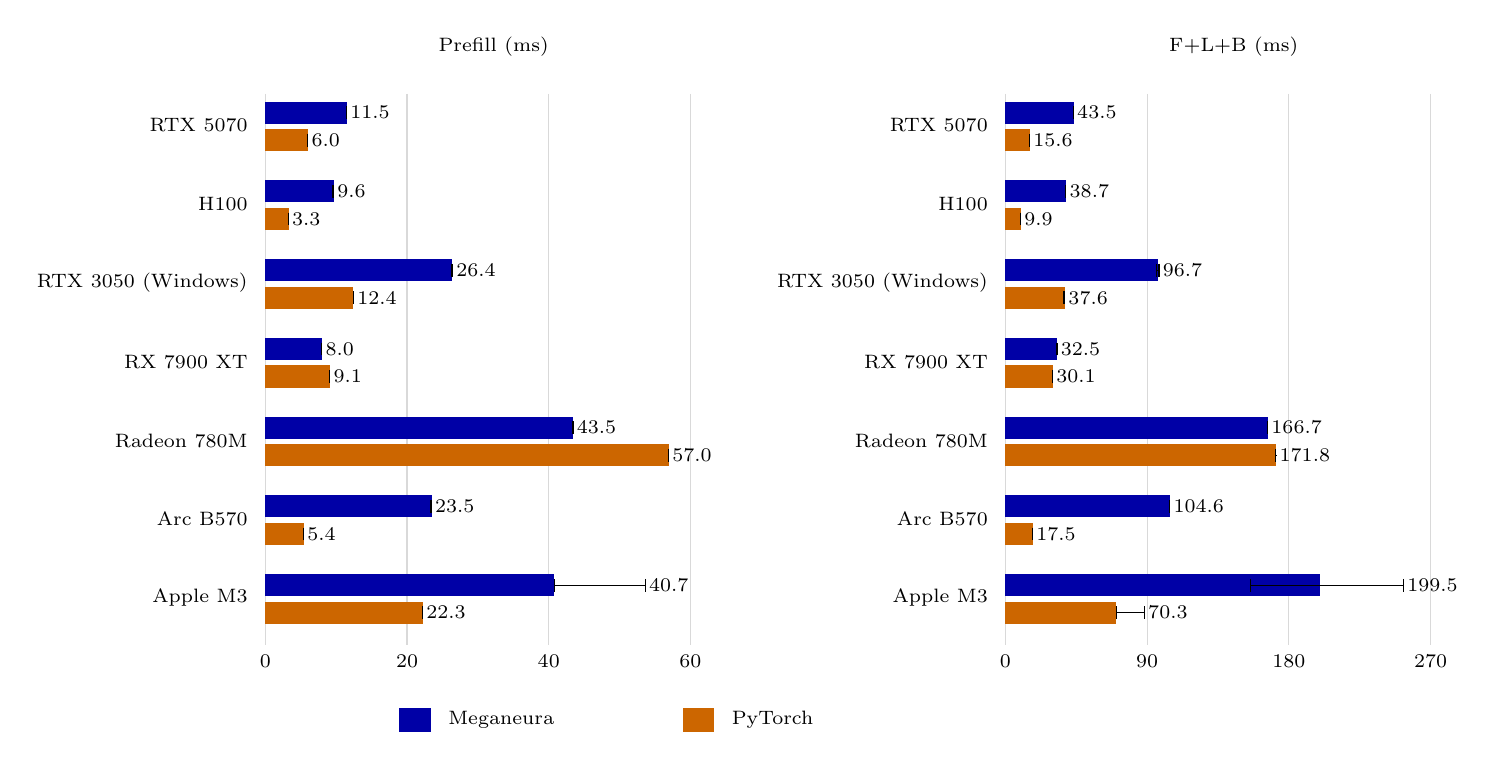
\begin{tikzpicture}[x=1mm,y=1mm,font=\scriptsize]
\node at (61,7) {Prefill (ms)};
\draw[black!15] (32,1) -- (32,-69);
\node[below] at (32,-69) {0};
\draw[black!15] (50,1) -- (50,-69);
\node[below] at (50,-69) {20};
\draw[black!15] (68,1) -- (68,-69);
\node[below] at (68,-69) {40};
\draw[black!15] (86,1) -- (86,-69);
\node[below] at (86,-69) {60};
\node[anchor=east] at (31,-3) {RTX 5070};
\fill[blue!65!black] (32,0.0) rectangle (42.3860,-2.8);
\node[anchor=west,inner sep=1pt] at (42.3862,-1.4) {11.5};
\draw[black,|-|] (42.3478,-1.4) -- (42.3862,-1.4);
\fill[orange!80!black] (32,-3.5) rectangle (37.4310,-6.3);
\node[anchor=west,inner sep=1pt] at (37.4548,-4.9) {6.0};
\draw[black,|-|] (37.4287,-4.9) -- (37.4548,-4.9);
\node[anchor=east] at (31,-13) {H100};
\fill[blue!65!black] (32,-10.0) rectangle (40.6711,-12.8);
\node[anchor=west,inner sep=1pt] at (40.7203,-11.4) {9.6};
\draw[black,|-|] (40.6454,-11.4) -- (40.7203,-11.4);
\fill[orange!80!black] (32,-13.5) rectangle (34.9851,-16.3);
\node[anchor=west,inner sep=1pt] at (34.9913,-14.9) {3.3};
\draw[black,|-|] (34.9851,-14.9) -- (34.9913,-14.9);
\node[anchor=east] at (31,-23) {RTX 3050 (Windows)};
\fill[blue!65!black] (32,-20.0) rectangle (55.7487,-22.8);
\node[anchor=west,inner sep=1pt] at (55.8421,-21.4) {26.4};
\draw[black,|-|] (55.7480,-21.4) -- (55.8421,-21.4);
\fill[orange!80!black] (32,-23.5) rectangle (43.1786,-26.3);
\node[anchor=west,inner sep=1pt] at (43.2671,-24.9) {12.4};
\draw[black,|-|] (43.1380,-24.9) -- (43.2671,-24.9);
\node[anchor=east] at (31,-33) {RX 7900 XT};
\fill[blue!65!black] (32,-30.0) rectangle (39.2356,-32.8);
\node[anchor=west,inner sep=1pt] at (39.2398,-31.4) {8.0};
\draw[black,|-|] (39.2077,-31.4) -- (39.2398,-31.4);
\fill[orange!80!black] (32,-33.5) rectangle (40.1541,-36.3);
\node[anchor=west,inner sep=1pt] at (40.2577,-34.9) {9.1};
\draw[black,|-|] (40.1307,-34.9) -- (40.2577,-34.9);
\node[anchor=east] at (31,-43) {Radeon 780M};
\fill[blue!65!black] (32,-40.0) rectangle (71.1187,-42.8);
\node[anchor=west,inner sep=1pt] at (71.1516,-41.4) {43.5};
\draw[black,|-|] (71.0931,-41.4) -- (71.1516,-41.4);
\fill[orange!80!black] (32,-43.5) rectangle (83.2587,-46.3);
\node[anchor=west,inner sep=1pt] at (83.2674,-44.9) {57.0};
\draw[black,|-|] (83.2280,-44.9) -- (83.2674,-44.9);
\node[anchor=east] at (31,-53) {Arc B570};
\fill[blue!65!black] (32,-50.0) rectangle (53.1181,-52.8);
\node[anchor=west,inner sep=1pt] at (53.1339,-51.4) {23.5};
\draw[black,|-|] (53.1026,-51.4) -- (53.1339,-51.4);
\fill[orange!80!black] (32,-53.5) rectangle (36.8985,-56.3);
\node[anchor=west,inner sep=1pt] at (36.9269,-54.9) {5.4};
\draw[black,|-|] (36.7886,-54.9) -- (36.9269,-54.9);
\node[anchor=east] at (31,-63) {Apple M3};
\fill[blue!65!black] (32,-60.0) rectangle (68.6441,-62.8);
\node[anchor=west,inner sep=1pt] at (80.3299,-61.4) {40.7};
\draw[black,|-|] (68.6372,-61.4) -- (80.3299,-61.4);
\fill[orange!80!black] (32,-63.5) rectangle (52.0292,-66.3);
\node[anchor=west,inner sep=1pt] at (52.0295,-64.9) {22.3};
\draw[black,|-|] (52.0073,-64.9) -- (52.0295,-64.9);
\node at (155,7) {F+L+B (ms)};
\draw[black!15] (126,1) -- (126,-69);
\node[below] at (126,-69) {0};
\draw[black!15] (144,1) -- (144,-69);
\node[below] at (144,-69) {90};
\draw[black!15] (162,1) -- (162,-69);
\node[below] at (162,-69) {180};
\draw[black!15] (180,1) -- (180,-69);
\node[below] at (180,-69) {270};
\node[anchor=east] at (125,-3) {RTX 5070};
\fill[blue!65!black] (126,0.0) rectangle (134.6905,-2.8);
\node[anchor=west,inner sep=1pt] at (134.6941,-1.4) {43.5};
\draw[black,|-|] (134.6830,-1.4) -- (134.6941,-1.4);
\fill[orange!80!black] (126,-3.5) rectangle (129.1143,-6.3);
\node[anchor=west,inner sep=1pt] at (129.1155,-4.9) {15.6};
\draw[black,|-|] (129.1138,-4.9) -- (129.1155,-4.9);
\node[anchor=east] at (125,-13) {H100};
\fill[blue!65!black] (126,-10.0) rectangle (133.7303,-12.8);
\node[anchor=west,inner sep=1pt] at (133.7383,-11.4) {38.7};
\draw[black,|-|] (133.6531,-11.4) -- (133.7383,-11.4);
\fill[orange!80!black] (126,-13.5) rectangle (127.9748,-16.3);
\node[anchor=west,inner sep=1pt] at (127.9827,-14.9) {9.9};
\draw[black,|-|] (127.9675,-14.9) -- (127.9827,-14.9);
\node[anchor=east] at (125,-23) {RTX 3050 (Windows)};
\fill[blue!65!black] (126,-20.0) rectangle (145.3421,-22.8);
\node[anchor=west,inner sep=1pt] at (145.5756,-21.4) {96.7};
\draw[black,|-|] (145.0961,-21.4) -- (145.5756,-21.4);
\fill[orange!80!black] (126,-23.5) rectangle (133.5219,-26.3);
\node[anchor=west,inner sep=1pt] at (133.5836,-24.9) {37.6};
\draw[black,|-|] (133.5061,-24.9) -- (133.5836,-24.9);
\node[anchor=east] at (125,-33) {RX 7900 XT};
\fill[blue!65!black] (126,-30.0) rectangle (132.5095,-32.8);
\node[anchor=west,inner sep=1pt] at (132.6060,-31.4) {32.5};
\draw[black,|-|] (132.5005,-31.4) -- (132.6060,-31.4);
\fill[orange!80!black] (126,-33.5) rectangle (132.0205,-36.3);
\node[anchor=west,inner sep=1pt] at (132.0303,-34.9) {30.1};
\draw[black,|-|] (132.0118,-34.9) -- (132.0303,-34.9);
\node[anchor=east] at (125,-43) {Radeon 780M};
\fill[blue!65!black] (126,-40.0) rectangle (159.3302,-42.8);
\node[anchor=west,inner sep=1pt] at (159.3594,-41.4) {166.7};
\draw[black,|-|] (159.3211,-41.4) -- (159.3594,-41.4);
\fill[orange!80!black] (126,-43.5) rectangle (160.3670,-46.3);
\node[anchor=west,inner sep=1pt] at (160.4026,-44.9) {171.8};
\draw[black,|-|] (160.2527,-44.9) -- (160.4026,-44.9);
\node[anchor=east] at (125,-53) {Arc B570};
\fill[blue!65!black] (126,-50.0) rectangle (146.9192,-52.8);
\node[anchor=west,inner sep=1pt] at (146.9287,-51.4) {104.6};
\draw[black,|-|] (146.9082,-51.4) -- (146.9287,-51.4);
\fill[orange!80!black] (126,-53.5) rectangle (129.4956,-56.3);
\node[anchor=west,inner sep=1pt] at (129.5057,-54.9) {17.5};
\draw[black,|-|] (129.4773,-54.9) -- (129.5057,-54.9);
\node[anchor=east] at (125,-63) {Apple M3};
\fill[blue!65!black] (126,-60.0) rectangle (165.8965,-62.8);
\node[anchor=west,inner sep=1pt] at (176.6175,-61.4) {199.5};
\draw[black,|-|] (157.0255,-61.4) -- (176.6175,-61.4);
\fill[orange!80!black] (126,-63.5) rectangle (140.0623,-66.3);
\node[anchor=west,inner sep=1pt] at (143.7123,-64.9) {70.3};
\draw[black,|-|] (140.0615,-64.9) -- (143.7123,-64.9);
\fill[blue!65!black] (49,-80) rectangle (53,-77);
\node[anchor=west] at (54,-78.5) {Meganeura};
\fill[orange!80!black] (85,-80) rectangle (89,-77);
\node[anchor=west] at (90,-78.5) {PyTorch};
\end{tikzpicture}
}
\caption{Strict SmolLM2-135M wall times on the six GPU-reference systems.
Bars are medians of three process medians.
Whiskers show the observed process range, not confidence intervals.
All native sessions enable tuning;
all references compile, with replay on CUDA/HIP/XPU.
Prefill and F+L+B have separate linear axes because these are distinct
workloads, not additive phases or CPU/GPU partitions.}
\label{fig:smollm2}
\end{figure*}

\subsection{Performance under bounded preparation}

Across the six platforms, median strict ratios are 1.27 for inference,
1.09 for minimal shapes, and 1.92 for training. Meganeura is nominally
faster in 7/30, 12/29, and 4/29 comparisons. The accelerated ratios are
2.00, 1.27, and 2.61, with 6/30, 10/29, and 4/29 nominal wins.
Only PyTorch's RX~7900~XT Whisper minimal/training timings are missing,
under both contracts. Meganeura's qualified times remain in the table.
This is a numerical portability failure in PyTorch's ROCm path, not a
disqualification of the GPU or Meganeura. Ratio medians include only
qualified pairs; a failed reference is not an infinite speedup.

RX~7900~XT is Meganeura's strongest paired platform. Strict SmolLM2,
SmolVLA, and diffusion are faster in all three phases; Whisper inference
is also faster. SmolLM2 and SmolVLA minimal-shape ratios are 0.19 and
0.22, and SmolVLA training is 0.48. Arc~B570 has the opposite pattern:
PyTorch wins every phase, with strict inference ratios of 1.76--2.62
and training ratios of 2.50--5.07.

On RTX~5070, strict diffusion and ResNet inference ratios are 0.91 and
0.74. SmolLM2 prefill is 1.20 and its one-token forward is 0.92;
SmolVLA inference is close at 1.09. Training still takes 1.60--2.40
times as long. Windows RTX~3050 completes all 30 pairs; strict inference
ratios span 1.16--1.64 and training 1.63--2.18.
We did not profile or hand-optimize kernels specifically for H100 before
collection. It tests how the shared implementation transfers to a
datacenter GPU, not the best performance an H100-specific implementation
could reach.
Strict training ratios span 1.49--3.43; accelerated ratios span 2.42--7.36.
Accelerated ResNet has the largest gap. These engine/driver results
cannot, by themselves, attribute that difference to barriers or one
instruction family.

M3 needs more caution. Diffusion has lower medians in both contracts, but many
process ranges are wide in both engines. Strict SmolVLA inference spans
28.59--49.77\,ms native and 8.95--40.35\,ms PyTorch; native strict
one-token SmolLM2 spans 6.88--43.11\,ms. All checks pass, but these are
noisy timing observations, not precise estimates of an M3-wide advantage.
The operator reports possible sleep interruptions. A post-hoc sensitivity
check drops samples above three times their own process median, applying
the same rule to both engines. It removes five of 3,600 samples, changes no
inference aggregate, and changes only one training aggregate by 2.5\%.
The broad variation is not just isolated spikes. We retain the original
medians and ranges; the records cannot separate machine state from
variation in selected implementations.

\subsection{What compile-time search actually explores}
\label{sec:search}

\begin{table*}[t]
\caption{Native search in the 180 main-matrix processes, summed across
both contracts. This includes the six partial reference pairs.}
\label{tab:search}
\centering
\small
\setlength{\tabcolsep}{5pt}
\begin{tabular}{llrrrrrrr}
\toprule
Device & Workload & \multicolumn{3}{c}{PyTorch replay gain} & \multicolumn{2}{c}{Search inf. gain} & \multicolumn{2}{c}{Compile seconds: light/searched} \\ & & Inf. & Min. & F+L+B & M & P & M & P \\
\midrule
RTX 5070 & SmolLM2-135M & 1.06 & 1.64 & 1.04 & 1.09 & 1.00 & 0.88/1.12 & 46.69/72.75 \\
 & SmolVLA & 1.09 & 1.44 & 1.08 & 1.00 & 1.00 & 0.79/1.06 & 24.05/49.76 \\
 & StableDiffusion & 1.13 & 1.11 & 1.46 & 1.04 & 1.09 & 0.48/1.83 & 29.78/124.25 \\
 & ResNet-50 & 1.02 & 1.04 & 1.02 & 1.07 & 1.23 & 0.54/5.09 & 13.26/58.25 \\
 & Whisper-tiny & 1.03 & 1.03 & 1.02 & 1.00 & 1.00 & 0.45/2.25 & 7.09/30.18 \\
H100 & SmolLM2-135M & 1.39 & 2.74 & 2.24 & 1.36 & 1.00 & 1.22/1.61 & 55.73/259.38 \\
 & SmolVLA & 1.35 & 1.68 & 3.06 & 1.10 & 1.27 & 0.99/1.52 & 33.97/163.44 \\
 & StableDiffusion & 1.49 & 1.54 & 3.55 & 1.08 & 1.08 & 0.69/2.81 & 29.69/592.06 \\
 & ResNet-50 & 1.18 & 1.24 & 1.21 & 1.20 & 1.28 & 0.77/6.16 & 14.09/601.27 \\
 & Whisper-tiny & 1.17 & 1.24 & 1.48 & 1.06 & 0.91 & 0.67/2.64 & 7.84/192.13 \\
\bottomrule
\end{tabular}

\end{table*}

Table~\ref{tab:search} counts 504 native sessions trying 19,696 programs.
In 169 sessions the selected graph/schedule differs from ordinary
extraction. Program search is unfinished in 459 sessions; the longest
takes 64.39\,s against the soft 60-second deadline. Extraction separately
reports truncation in 396 sessions. None reports a skipped region.
This is bounded search, not exhaustive optimization.

Across program trials, private probes visit or reuse results for 291,436
of 293,310 eligible kernel-class instances. Repeated classes and reused
comparisons mean these counts are not distinct algorithms. There are
7,133 accepted kernel replacements, 3,214 kernel-output rejections, and
725 whole-program
output rejections. Rejected candidates cannot replace the checked winner.
An accepted local change is not proof of an end-to-end speedup over another
compiler revision or under a later machine state.

The kernel domain includes scalar matrix multiplication, supported
native-f32 cooperative tiles, matrix--vector multiplication (GEMV),
reductions, and convolution shape/staging choices. Reduced-input
cooperative paths are available, but are not exhaustively tuned.
Graph alternatives come from the existing rewrite rules; the search
does not invent new kernel algorithms. M3 records 2,364 cooperative
dispatch instances in strict mode. B570's driver exposes rectangular
$8\times16\times16$ floating-point tiles, but this Blade/Naga path accepts
only square tiles \cite{blade2026matrices}. B570 therefore uses no cooperative
dispatches in either contract. That is a limit of this implementation, not
of the Intel hardware.

\subsection{What the e-graph contributes}
\label{sec:egraph-ablation}

The e-graph keeps graph rewrites and matrix schedules available for the
same measured search. A layout or fusion choice need not be discarded
before its tile and split-reduction alternatives have been tested.
This avoids treating the cheapest estimated graph as the only graph
worth tuning.

The 169 changed selections in Table~\ref{tab:search} show that the measured
path uses these alternatives. They do not measure a speedup over a greedy
optimizer: this cohort has no greedy or search-off arm at the same revision.
Nor does the e-graph itself improve a kernel. The benefit depends on which
implementations it can express, how it orders them, and what the budget
allows it to measure. The current byte-traffic estimate is a search guide,
not an execution-time model.

\subsection{Larger models}
\label{sec:scaling}

\begin{table*}[t]
\caption{Same-revision SmolLM2 size study. Every entry is the median of
three process medians; M and P denote Meganeura and PyTorch.}
\label{tab:scaling}
\centering
\footnotesize
\setlength{\tabcolsep}{4.5pt}
\begin{tabular}{lllrrrrrr}
\toprule
Device & Model & Arithmetic & \multicolumn{2}{c}{Prefill ms} & \multicolumn{2}{c}{One token ms} & \multicolumn{2}{c}{F+L+B ms} \\ & & & M & P & M & P & M & P \\
\midrule
RTX 5070 & 135M & strict & 7.29 & 6.08 & 1.51 & 1.64 & 31.94 & 15.60 \\
RTX 5070 & 135M & accelerated & 7.52 & 2.73 & 1.52 & 1.64 & 30.79 & 9.56 \\
RTX 5070 & 360M & strict & 19.94 & 11.82 & 4.45 & 3.18 & 60.41 & 28.64 \\
RTX 5070 & 360M & accelerated & 17.23 & 5.01 & 4.45 & 3.18 & 57.09 & 16.67 \\
RX 7900 XT & 135M & strict & 6.14 & 9.20 & 1.18 & 6.19 & 26.92 & 30.56 \\
RX 7900 XT & 135M & accelerated & 7.40 & 9.20 & 1.18 & 6.19 & 26.01 & 30.67 \\
RX 7900 XT & 360M & strict & 12.07 & 17.14 & 2.57 & 10.04 & 42.68 & 49.48 \\
RX 7900 XT & 360M & accelerated & 13.87 & 17.18 & 2.57 & 10.05 & 41.45 & 49.62 \\
H100 & 135M & strict & 6.06 & 3.30 & 1.29 & 1.28 & 32.20 & 9.92 \\
H100 & 135M & accelerated & 8.07 & 2.16 & 1.29 & 1.28 & 29.92 & 6.86 \\
H100 & 360M & strict & 9.82 & 5.10 & 2.13 & 1.84 & 44.51 & 15.02 \\
H100 & 360M & accelerated & 14.02 & 2.80 & 2.17 & 1.84 & 44.24 & 9.14 \\
H100 & 1.7B & strict & 29.90 & 11.87 & 7.13 & 3.24 & 99.80 & 35.84 \\
H100 & 1.7B & accelerated & 53.58 & 4.37 & 7.27 & 3.24 & 107.78 & 16.39 \\
\bottomrule
\end{tabular}

\end{table*}

Table~\ref{tab:scaling} extends the same protocol and source pins to
360M on RTX~5070, RX~7900~XT, and H100, and 1.7B on H100.
All 24 larger-model pairs pass. They do not enter the five-workload
aggregate, and no earlier cohort is needed to complete the size series.
The H100 extension uses a different cloud allocation from the 135M baseline:
GPU UUID and host kernel differ, while GPU model, memory, driver and software
pins match. The 360M and 1.7B rows share that second allocation. This is a
comparison across matching GPUs, not a controlled same-host scaling test.

On H100, strict training ratios narrow
3.25$\rightarrow$2.96$\rightarrow$2.78 from 135M through 360M to 1.7B.
Inference moves in the opposite direction: prefill ratios grow
1.84$\rightarrow$1.93$\rightarrow$2.52, and one-token ratios grow
1.01$\rightarrow$1.15$\rightarrow$2.20. Larger weights do not simply
amortize a fixed submission cost. Accelerated training widens
4.36$\rightarrow$4.84$\rightarrow$6.58; accelerated 1.7B prefill is
$12.26\times$ PyTorch's. Native accelerated prefill itself takes longer
than strict (53.58 versus 29.90\,ms). Permitting a cooperative path and
searching the current alternatives does not ensure a faster result.

The desktop results are also platform-dependent. On RTX~5070, strict
prefill grows from 1.20 to 1.69 times PyTorch, and the one-token forward
goes from 0.92 to 1.40. RX~7900~XT keeps its advantage at 360M:
strict prefill, one-token, and training ratios are 0.70, 0.26, and 0.86.
B570's first 360M attempt fails in PyTorch embedding backward during XPU
graph capture. Native execution completes its own checks, but without a
qualified independent reference that attempt supplies no paired timing.
Architecture and shape also change between variants. These are
small-batch, short-context scaling observations, not a fitted scaling
law or a production LLM serving/training benchmark.

\subsection{Performance portability on the declared platform set}

\begin{table}[t]
\caption{Strict scores over all six main platforms. Missing qualified\nPyTorch phases receive zero; native-only qualified timings remain included.}
\label{tab:pp}
\centering
\small
\setlength{\tabcolsep}{4pt}
\begin{tabular}{lrrrrrr}
\toprule
Workload & \multicolumn{2}{c}{Inference} & \multicolumn{2}{c}{Minimal} & \multicolumn{2}{c}{F+L+B} \\ & M & P & M & P & M & P \\
\midrule
SmolLM2-135M & 0.43 & 0.94 & 0.72 & 0.60 & 0.39 & 0.98 \\
SmolVLA & 0.51 & 0.89 & 0.73 & 0.63 & 0.46 & 0.90 \\
StableDiffusion & 0.53 & 0.85 & 0.54 & 0.85 & 0.49 & 1.00 \\
ResNet-50 & 0.59 & 0.97 & 0.58 & 0.95 & 0.35 & 1.00 \\
Whisper-tiny & 0.48 & 0.94 & 0.51 & 0.94 & 0.36 & 0.99 \\
Workload mean & 0.51 & 0.92 & 0.62 & 0.79 & 0.41 & 0.97 \\
\bottomrule
\end{tabular}

\end{table}

For workload $a$, phase $q$, implementation $i$, and declared machine
set $S$, application efficiency is
$e_{i,a,q}(p)=t_{\mathrm{best\ valid},a,q}(p)/t_{i,a,q}(p)$.
We use the Pennycook metric \cite{pennycook2016metric,pennycook2021revisiting}:
\begin{equation}
P_{i,a,q}=\begin{cases}
|S|\big/\sum_{p\in S}1/e_{i,a,q}(p),&\text{valid on every }p,\\
0,&\text{otherwise.}
\end{cases}
\end{equation}
Best means the fastest qualified result of these two engines under the
declared policies, requiring three processes for a timing entry.
Table~\ref{tab:pp} keeps all six main platforms for every workload and phase.
If only one engine qualifies on a platform, its efficiency there is one;
this is the best \emph{available} result, not a claimed speedup over the
failed engine. The final row is the arithmetic mean of the five workload
scores, not a new harmonic aggregate over applications.
Meganeura/PyTorch means are 0.64/0.90 for inference, 0.76/0.56 for minimal
shapes, and 0.48/0.74 for training (rounded).

RX~7900~XT stays in the declared set. PyTorch's failed Whisper training
and unreached minimal timing give it zero for those workload/phase scores.
The latter means the campaign supplied no qualified result, not that
standalone minimal inference is known to be unsupported. Meganeura's
independently qualified times remain valid.
The CPU-oracle qualifications, larger-model extension and MI300X lie
outside this six-platform score; it is not universal support.
If support is required across every attempted GPU, both stacks have a
known hole and hence a zero score: PyTorch on RPL-U, Meganeura on MI300X.
Availability therefore belongs alongside the timing ratios.

\section{Edge Deployment Beyond the Matrix}
\label{sec:edge}

The matched matrix contains no Android reference, so Android contributes no
performance-portability score. A separately versioned physical deployment
tests the stack in an interactive edge application. DinoVision reconstructs
the headset cameras' live images from features computed by a vision encoder
(DINOv3~\cite{simeoni2025dinov3}). Figure~\ref{fig:dinovision} shows the
reconstructed view displayed on the headset. \system{} trains
a 2.01-million-parameter decoder on a host GPU, saves its parameters, and
loads them into a joined batch-one encoder/decoder graph on a Quest~3S. The
deployed graph performs 2.359 billion multiply--accumulates and runs
through the same graph representation,
compiler, memory planner, checkpoint format, and Blade runtime. Two
asynchronous eye sessions share Blade's Vulkan context and queue with the
OpenXR renderer.
This shared context also makes hybrid applications straightforward:
games and interactive visualizations can combine rendering and ML without
introducing a separate vendor ML context. Resource sharing and queue
scheduling become application-level choices within one graphics stack.

\begin{figure}[t]
  \centering
  
\includegraphics[width=0.73\columnwidth]{../figures/dinovision-quest3s.jpg}
  \caption{Quest~3S casting capture of DinoVision's live RGB
  reconstruction. This documents physical deployment; it is not a visual
  quality or capture-to-photon benchmark.}
  \label{fig:dinovision}
\end{figure}

We ask two separate questions: does the deployed graph reproduce the host
output, and how does its GPU work affect the renderer sharing the queue?
The first has an independent host/device gate. For one fixed public
RGB frame and identical weights, preprocessed patches are bit-exact; Quest
encoder output has relative $L_2=0.001059$ and the final reconstruction has
relative $L_2=0.000457$ against the host. An isolated synchronized run takes
96.78\,ms as one submission chunk. Splitting the ordered dispatch plan into
two chunks costs 4.1\% in isolation, but under a 90-second live stereo sweep
it raises application render submissions by 18.8\%, raises the lower-eye
update rate by 8.7\%, and reduces median worker latency by 20.2\%. Larger
chunk counts regress non-monotonically. The best schedule here differs
between isolated inference and a shared rendering queue. A common graphics
stack lets the application make that choice without a second GPU runtime.

This case study shows a complete deployment sharing its queue with rendering,
not on-device training or speedup over PyTorch on Android. Its weights, raw
samples, manifests, and full-resolution media are available in the public
\href{https://huggingface.co/mad-bot/dinovision/tree/2c3f9017fe74c41482b165890c14737a2ccd4b6a}{DinoVision evidence
archive}; its \href{https://github.com/kvark/dinovision/tree/dc35cdf1c7c910cdd93c5b5362846842ae469a21}{source code} is
public as well.

\section{Locating the Gaps}
\label{sec:gaps}

The cohort measures synchronized wall time, not a kernel-by-kernel
decomposition. It establishes where the gap is large, but cannot assign
a percentage to command recording, barriers, or a particular instruction.

Meganeura's calibrated timestamps align CPU and GPU events. Optional
per-dispatch timing can locate expensive passes, while Nsight Systems
and Nsight Graphics can inspect GPU activity, occupancy, and stalls.
Per-dispatch instrumentation changes pass boundaries, so its cost must be
measured against the ordinary grouped schedule. Grouped spans include
inter-kernel gaps; summed kernel intervals may overlap. Neither can be
subtracted from wall time to obtain a CPU or barrier partition.

There are several concrete implementation limits to investigate. Small-output,
long-reduction products need enough workgroups to occupy the GPU; adding tile
choices alone may not provide that parallelism. The current search includes
split reductions, convolution indexing/staging choices, GEMV geometry, and
fused/unfused graph forms. Most sessions still reach their search limit.
Which candidates get measured matters as much as how many are expressible.

Token execution also includes command recording on the CPU. A low CPU
clock can increase that cost even when the GPU work is unchanged. Low CPU
demand makes downclocking a reasonable power-management response, not
necessarily a malfunction; its latency and energy effects need separate
measurement. It does not justify dropping slower cohort samples.

Strict 135M one-token execution is near PyTorch on 5070 and H100, but
takes $2.12\times$ as long on B570. The 360M and 1.7B results show that
small-model parity does not transfer to larger weights. The larger H100
inference gap calls for profiling those shapes, not extrapolating from
the smaller model.

Matrix instruction access may also contribute to the accelerated H100 gap.
Hopper's CUDA/PTX path exposes asynchronous matrix operations across a
128-thread warpgroup (\code{wgmma}), with explicit issue and completion
control \cite{nvidia2026wgmma}. The measured Blade/Naga Vulkan path accepts
only subgroup-scope $8\times8$ or $16\times16$ tiles
\cite{blade2026matrices}; it does not expose that programming model.
Vulkan's vendor extension \code{VK\_NV\_cooperative\_matrix2} adds workgroup
scope and more flexible dimensions, but this stack does not use it
\cite{khronos2024cooperative2}. This is a possible implementation/capability
gap. Determining its contribution requires inspecting matched-precision
machine code on H100; these measurements establish neither a specific
instruction deficit nor a fundamental Vulkan limit.

The results establish no removable Vulkan-barrier percentage. Workgroup
barriers inside shaders, resource dependencies between dispatches, host
submission, and waiting are different mechanisms. The companion
synchronization study explains why barrier policy matters
\cite{malyshau2026barriers}, but predates the present resource tracking.
We do not reuse its timings to explain the final cohort.
Matched-revision native profiles are needed for that attribution.

\section{Deployment Efficiency and Programmer Productivity}
\label{sec:productivity}

\subsection{Preparation as a deployment budget}

Native \code{compile\_s} covers graph construction, optimization,
autodiff, pipeline creation, representative initialization, numerical
qualification, and search across the requested sessions. Most models construct three sessions;
Whisper reuses one inference session for its two timing shapes.
PyTorch \code{compile\_s} includes compilation and the first
specializations/executions of forward, backward, and minimal shapes,
including on MPS.
PyTorch graph preparation and full-tensor qualification are recorded
separately. File loading, cross-engine validation, and other process
startup are outside these fields. These components do not add up to a
complete application time to first answer.

\begin{table*}[t]
\caption{Cumulative preparation costs in minutes; both contracts and all replicates.}
\label{tab:preparation}
\centering
\small
\setlength{\tabcolsep}{5pt}
\begin{tabular}{llrrrrr}
\toprule
Device & Policy & Pairs & M compile (s) & P compile (min) & P capture (s) & P qualification (s) \\
\midrule
RTX 5070 & light & 30 & 27.4 & 12.0 & 3.1 & 46.4 \\
RTX 5070 & searched & 30 & 46.4 & 33.0 & 3.1 & 46.4 \\
H100 & light & 30 & 102.5 & 15.1 & 6.0 & 294.0 \\
H100 & searched & 30 & 125.0 & 194.1 & 7.3 & 295.7 \\
\bottomrule
\end{tabular}

\end{table*}

Table~\ref{tab:preparation} sums the retained costs of all 180 main-matrix
attempts. H100 spends 72.81 minutes in native preparation versus 16.86
in default PyTorch compilation. Across the 30 strict workload/device
groups, process-median preparation spans 79.87--185.59\,s native and
2.19--83.95\,s PyTorch; the medians are 127.90 and 26.73\,s.
The six partial Whisper reference records contribute only their reported
costs. Eager diagnostics and hard-failed campaigns are not charged to
successful compiled preparation, so this is not total collection wall time.
Completed reference compilations remain below the 120-second deadline.

The native search is expensive. Across the main matrix, candidate
construction accounts for 80.99 cumulative minutes, private kernel search
for 122.45, initialization for 40.20, and full-program qualification
callbacks for 59.44. Much of this work is allocation, transfer, and
checking, not shader translation. A small shader compiler does not make
repeated whole-model construction cheap. H100's 1.7B preparation takes
211.06\,s strict and 216.69\,s accelerated, versus 40.10 and 40.56\,s
for default PyTorch compilation.
These costs are measured, not inferred from the nominal deadline.

Shader translation is only one part of preparing a candidate. Naga
processing does not include native driver machine-code compilation,
allocation, initialization, or numerical checks. Comparing its duration
alone with a complete Triton compilation would compare different stages.
The costs above cover the actual preparation policy used for these results.

Compile-time autotuning is established practice
\cite{chen2018tvm,tillet2019triton}. Meganeura brings it into a compact
deployment runtime, alongside graph compilation. The opportunity is real,
but the current search spends too much on repeated construction and checking
to make cheap startup a general claim. Better reuse and search allocation
matter as much as compiling individual shaders quickly.

\subsection{Availability is part of portability}
\label{sec:availability}

On Intel RPL-U, Meganeura runs all five workloads through Vulkan and
passes both arithmetic contracts. The pinned PyTorch stack provides no
usable GPU path there. The Ryzen~9600X integrated Radeon also passes
all ten conditions against eager CPU PyTorch. Its native adapter reports
\code{RADV RAPHAEL\_MENDOCINO}, device ID 5056; we identify the hardware
by the processor and adapter, not by treating that shared driver name as
a separate Mendocino product.
Reported ROCm bring-up on this device fails without an architecture
override and produces incorrect reference outputs with one. These are
GPU availability findings, not CPU-versus-GPU speedups.
Table~\ref{tab:qualification} separates that coverage from paired timings.

Arc~B570 provides the separate, working XPU comparison.
Its pinned native dense embedding backward passes only 19,968 of
73,728 expected elements in the shape-derived exact probe.
The harness therefore selects and records PyTorch's equivalent dense
\code{index\_add} autograd formulation; all 73,728 probe elements pass.
The 135M pairs validate with this workaround. At 360M, compilation completes
in 89.62\,s but training capture fails in
\path{aten.embedding_dense_backward} with an event-wait error. Passing the
small-model probe did not establish support for this larger workload.
Fused XPU SDPA also failed capture with an event-wait error during
qualification; the public math SDPA setting passes forward/backward replay
and is recorded for XPU. Neither workaround changes tolerances or disables
graph replay.
During bring-up, requested max-autotune did not finish its first ResNet
qualification within an hour. Default compilation supplies a working
bounded-preparation path.

On the Radeon~780M, bring-up required an architecture override
(\code{HSA\_OVERRIDE\_GFX\_VERSION=11.0.2}) and disabling asynchronous copies
(\code{HSA\_ENABLE\_SDMA=0}); both are recorded in the final manifest.
During bring-up on both Radeon machines, requested max-autotune failed
while compiling diffusion training: convolution candidates exceeded
local-memory limits or timed out, and the remaining library fallback
was invoked without its required output buffer.
The final 780M campaign fails on its first strict 135M condition under
default compilation: PyTorch reports an unspecified HIP launch failure.
Meganeura completes, but no paired timing is admitted. A separate Vulkan
qualification then passes all ten conditions against the CPU oracle.
This is a failure of the tested GPU reference path, not a claim that every
PyTorch configuration must fail on this hardware.
The ROCm-specific overrides and failures are a concrete portability cost;
the Vulkan path does not need those overrides. Windows, meanwhile,
completes all 30 pairs through Vulkan and compiled, replayed CUDA.
Earlier max-autotune findings are separate from these current records.\footnote{\href{https://github.com/kvark/inferena/blob/7b8fcb72e55410d8e33bbe948f89be50c691fcf7/EXPERIMENT.md}{Inferena protocol and bring-up notes, revision \code{7b8fcb72}}.}

RX~7900~XT exposes a numerical portability failure in default-compiled
PyTorch 2.13.0/ROCm 7.2. All six Whisper training processes fail on the
first uncaptured repeat, before HIP graph capture. Identical calls differ
by $1.84$--$2.45\times10^{-3}$ at the worst output element, against a
$9.10\times10^{-6}$ bound. Captured inference passes in all six.
Each separate eager/math diagnostic passes full-tensor repeatability and
agrees with the native gradients; parameter-norm-vector error stays below
0.001\%. This points to the compiled reference path, not a setup failure
or a reason to weaken validation. The exact kernel fault remains unresolved.
Meganeura continues to produce qualified results on this GPU. Its native
training and minimal-shape times remain in Table~\ref{tab:performance}
alongside the failed reference, as do the qualified inference ratios.
This is a portability advantage of the tested Vulkan path. No eager
diagnostic time replaces a failed compiled time.

MI300X exposes a different boundary: driver availability for a
compute-focused accelerator. PyTorch/ROCm runs strict 135M on the attempted
cloud allocation, but no usable Vulkan driver stack supplies a validated
Meganeura run. Mesa's RADV targets graphics-capable GCN/RDNA hardware,
not this CDNA accelerator \cite{mesa2026radv}.
A custom driver/compute-queue trial reaches execution but fails on real
workloads. This identifies missing driver support, not evidence that
the required tensor computation is intrinsically unsuitable for Vulkan.
There is already upstream work in this direction. Mesa issue 13399 tracks
RADV support for CDNA, including experimental compute-only execution and
unresolved correctness and hardware-utilization problems
\cite{mesa2025cdna}. This could open a Vulkan path to MI300X, but it is
work in progress, not a driver we qualified. The obstacle is software
support, not an inherent mismatch between Vulkan compute and tensor math.

\subsection{Application authors and backend maintainers}

Application authors express tensor graphs and reuse checkpoints across
backends. Maintaining the runtime still requires WGSL, memory,
synchronization, and numerical expertise. A shared stack reduces the
number of implementations to maintain; it does not remove that work.
Eager PyTorch offers immediate tensor inspection, Python execution,
autograd hooks, and anomaly detection.
A static compiler can fuse away values or alias their storage, so
debugging may require preserved intermediates or a less optimized plan.
Meganeura can read named intermediates, map graph operations to dispatches,
locate the first nonfinite value, and run the same kernels eagerly.
These tools help separate rewrite, storage-reuse, and kernel bugs.
Running the same kernel eagerly is useful for debugging, but is not an
independent numerical reference.

Portable traces connect CPU work with GPU passes;
native tools remain necessary for instruction, occupancy, and stall analysis.
The XPU compatibility probes illustrate why such observability matters
even when broad regression gates pass.
We did not measure developer-hours, learnability, maintenance effort, or
equivalent independent ports, and claim no quantitative productivity advantage.

Native deployment does not require Python or the vendor ML runtime.
That simplifies embedding in an existing graphics application, but the
cohort does not measure installation footprint or equivalent feature
coverage. Section~\ref{sec:edge} supplies a physical application check.

\subsection{Memory accounting}

\begin{table}[t]
\caption{H100 size study: strict memory accounting (GiB), $n=3$.}
\label{tab:memory}
\centering
\small
\setlength{\tabcolsep}{3pt}
\begin{tabular}{lrrrr}
\toprule
Model & $n$ & M plan & P allocated & P reserved \\
\midrule
SmolLM2-135M & 3 & 1.52 & 1.13 & 1.42 \\
SmolLM2-360M & 3 & 3.77 & 2.82 & 3.29 \\
SmolLM2-1.7B & 3 & 16.72 & 12.86 & 13.54 \\
\bottomrule
\end{tabular}

\end{table}

Table~\ref{tab:memory} reports the maximum recorded phase value per
process, then its median over $n$ processes. Meganeura's column counts
physical execution-plan allocations after lifetime aliasing; it excludes
driver overhead and is not a measured peak of resident device memory.
PyTorch's columns are caching-allocator allocated and reserved high-water
marks; phases share a process and retain earlier allocations.
These different scopes cannot establish a relative peak-VRAM advantage.
Meganeura also retains device-memory snapshots at phase boundaries, not
a continuous high-water mark. A matched process/device-memory peak
measurement would strengthen capacity and scaling analysis. H100's optional
NVIDIA Management Library (NVML) process-memory query is unavailable in
this allocation; CUDA device
identity, replay, and allocator peaks remain recorded. Missing monitoring
data are not replaced with zero or interpreted as CPU fallback.

\section{Related Work}

Pennycook et al.\ define and later revisit the portability metric used here
\cite{pennycook2016metric,pennycook2021revisiting}. Kokkos and RAJA encode
portable parallelism and memory policy in C++ libraries
\cite{edwards2014kokkos,beckingsale2019raja}; SYCL standardizes a
single-source heterogeneous C++ model~\cite{khronos2020sycl}. We instead
start from graphics APIs and build the tensor compiler above them.
Lin et al.\ measure programming-model productivity through semantic
divergence. Preparation time and binary size do not replace that
programmer-facing measure
\cite{lin2024productivity}.

TVM, Glow, MLIR, and Triton established graph and kernel compilation for ML
\cite{chen2018tvm,rotem2018glow,lattner2021mlir,tillet2019triton}; RAF
extends whole-graph compilation to training~\cite{yu2023raf}. Egglog supplies
the equality-saturation machinery used by our optimizer~\cite{zhang2023egglog}.
Burn~0.21 is a broader Rust framework: it supports compute and graphics
backends, autodiff, fusion, routing, and remote execution~\cite{simard2026burn}.
Its larger feature set makes binary size alone a poor comparison.
TensorFlow.js demonstrated
browser-resident training and inference~\cite{smilkov2019tensorflowjs}, and
systems for memory-constrained on-device training study a complementary
resource regime~\cite{lin2022ondevice}. Portable autodiff is not new.
Our contribution is the measured comparison of a compact native graphics
path across these devices, including its failures, preparation costs,
profiles, and physical deployment.
\inferena{} was built to compare such frameworks, including Rust-originating
systems such as Burn, Candle, Luminal, and Meganeura. This paper selects
PyTorch as its reference rather than claiming results for every runner
available in that harness.

TinyIREE measures artifact and runtime footprint for embedded
inference~\cite{liu2022tinyiree}; ExecuTorch deploys
exported PyTorch programs across mobile backends at scale
\cite{nachin2026executorch}. WebLLM and LlamaWeb demonstrate browser
graphics-API inference performance
\cite{ruan2024webllm,levine2026llamaweb}. \system{} carries the backward pass,
optimizer, and checkpoint through a native Vulkan/Metal stack.
The companion technical report gives the full
system and compiler account~\cite{malyshau2026meganeura}; the Blade study
isolates synchronization in the underlying graphics abstraction
\cite{malyshau2026barriers}.

\section{Threats to Validity}

A common PyTorch source revision does not equalize vendor libraries,
drivers, host CPUs, operating systems, or permitted fast paths.
All primary references compile; CUDA/HIP/XPU use qualified replay, while
MPS has no equivalent public whole-phase API. XPU's recorded embedding
and math-attention accommodations are not an unmodified stock execution path.
CPU-oracle qualification, the larger-model extension, and the earlier
MI300X attempt remain separate from the five-workload timing aggregate.
Both contracts have 30 qualified inference groups and 29 minimal/training
groups. The portability score keeps all six platforms and treats a
missing qualified phase as zero for that engine. It therefore combines
speed and availability; read it with the timing table, which distinguishes
PyTorch's failed training from its unreached minimal phase.

Every native session enables search and permits legal native-f32 tiles
in strict mode, but coverage is bounded by the implemented domain,
memory availability, and soft time limit. The cohort has no search-off
or cooperative-off arm at its final revision. It therefore measures
deployable policies, not an isolated causal effect of tuning or
cooperative matrices. Native per-session and reference compilation
budgets have different boundaries; neither identical startup cost nor
the fastest possible implementation is claimed.

The larger models have three processes under both contracts at the same
revisions as the main matrix. H100's 135M baseline and larger models use
different cloud allocations. They do not establish production LLM
performance: batch and sequence length remain small,
decoding has no cache, and training excludes optimizer state and distributed
communication. The diffusion graph is reduced, Whisper omits its decoder,
and ResNet uses inference-folded normalization.

Fresh processes have empty private TorchInductor/Triton caches, while
persistent driver and vendor-library state remains as found.
Alternating engine order mitigates rather than removes history dependence.
Preparation results describe installed systems, not independent first-use
cold starts. Disabling max-autotune does not clear a lower-level algorithm
choice established by earlier activity.

Three process replicates do not characterize a platform population.
CPU power policy, cloud co-tenancy, thermals, and timing-window length can
affect results. Process ranges are retained, including substantial M3
variation in both engines. The two-second/five-call minimum warmup followed
by 20 samples measures warmed short-window latency, not guaranteed
sustained throughput. No outlier was removed to improve a ratio, and the
data do not separate tuning-choice variation from changing machine state.

Strict f32 constrains permissions, not operation order or bitwise identity.
Qualification on one parameter distribution does not certify another.
Cross-engine sampled outputs and gradient norms can miss localized or sign
errors. Full-element replay qualification checks PyTorch against itself;
it does not turn the cross-engine gate into an elementwise gradient
comparison. All 198 complete GPU pairs and 30 qualification pairs
individually pass the 5\% gradient bound. The six partial pairs validate
native training only against a separate eager diagnostic, not the failed
compiled reference. Complete timing groups also pass the replicated rule.
Replay's fixed tensor maximum/RMS
bounds and their coefficients are explicit; pointwise mismatch counts are
diagnostics, not a second acceptance rule.

Planner allocation sizes, allocator reservations, and process/driver
accounting have different meanings. A host-visible Vulkan allocation can
also occupy device memory; the planner's device-local category does not
prove physical heap placement. The H100 extension is not a controlled
placement or PCIe study. Missing process-memory telemetry does not establish
a memory saving.

All framework timing comparisons use the final cohort; no earlier
profile or benchmark fills a missing entry. The separately versioned
DinoVision deployment and MI300X driver investigation address application
integration and availability, not paired performance.
Work on several vendors informed this compiler; the experiment does not
isolate general architecture from accumulated engineering.
Preparation time does not measure programmer productivity.

\section{Future Work}

The immediate work is to spend the search budget better: reuse initialized
weights and compilation work, prioritize expensive kernels, and make choices
that survive longer timing windows. B570 also needs support for rectangular
cooperative tiles. More search alone is not the answer.

With graph forms and schedules in the same search, the next question is
how to rank them cheaply. Logical tensor bytes alone cannot rank their
execution time. Reusing measured kernel-class costs could improve
search order without replacing the final whole-program comparison. That
empirical extraction model is not implemented yet.

Beyond GPU optimization, neural accelerators would need a backend for their
operator, layout, and precision constraints. Unsupported operations could
stay on the GPU, but the placement decision must include transfers,
synchronization, and numerical checks. The aim is one graph interface,
not a claim that all devices expose the same operations.

Persistent megakernels could move dependency scheduling onto the device,
reducing dispatch boundaries and some intermediate memory traffic. MPK
demonstrates automatic tensor-program lowering to persistent CUDA task
graphs~\cite{cheng2026mpk}. Applying this idea through graphics APIs raises
different portability questions: workgroup forward progress, residency,
cross-workgroup synchronization, and register pressure. A bounded search
could choose profitable regions while retaining the ordinary multi-kernel
schedule as a qualified baseline. Neither direction is an implemented or
measured capability of the present system.

\section{Conclusion}

Graphics APIs provide a useful ML deployment path. Meganeura qualifies
nine GPUs across Vulkan and Metal, including Windows and three integrated
GPUs without a qualified PyTorch GPU comparison. The main matrix keeps
180 inference pairs and 174 training pairs; a further 24 complete pairs
extend the same implementation to 360M and 1.7B models.

PyTorch is faster in most comparisons. Median strict inference and
training take $1.27\times$ and $1.92\times$ as long in Meganeura over
the qualified timing groups. RX~7900~XT shows that the graphics path can
win across several workloads; B570 shows how much kernel efficiency is
still missing. On H100, larger models narrow the strict training gap but
widen the inference gap. More weights do not make the difference disappear.

Joint graph and kernel search finds useful alternatives without
model-specific schedules, but it is bounded and preparation is expensive.
The next work is better kernel coverage and better use of that budget,
not simply more search. Correctness and availability belong beside speed:
compiled PyTorch fails Whisper repeatability on Radeon and larger-model
capture on Arc, while missing Vulkan support blocks our MI300X path.

\section*{Acknowledgments}

I thank my family for their support and patience throughout this work.

Anthropic Claude and OpenAI Codex/GPT
\cite{anthropic2026claude,openai2026codex} assisted code review,
benchmark-harness and instrumentation development, experimental debugging,
data analysis, and drafting and editing throughout all numbered sections and
the Artifact Description.
AI-generated draft passages were subsequently reviewed and revised.
Substantial portions of the \system{} and \inferena{} source code were also
developed with AI assistance under my direction and review. I designed the
study, directed the experiments and analysis, and accept full responsibility
for the content.

\bibliographystyle{IEEEtran}
\bibliography{../references,references}

\clearpage
\setcounter{section}{0}
\setcounter{subsection}{0}
\renewcommand{\theHsection}{AD.\arabic{section}}
\hypersetup{hidelinks}
\twocolumn[{%
\begin{center}
\Huge Appendix: Artifact Description
\end{center}
}]
% SC26 AD template, jennfshr/sc26-repro b5195e67d9ad0b5d07e8b6840558c7251c73b3c0.
% Included after the paper's references using the supplied IEEEtran/sc26repro style.
% No AE appendix or badge claim is submitted.
%\usetag{explanation}
%\usetag{example}
\appendixAD

\section{Overview of Contributions and Artifacts}

\subsection{Paper's Main Contributions}

\begin{description}
\item[$C_1$] A numerically checked comparison of a compact Vulkan/Metal
training and inference stack with compiled PyTorch on six GPUs from four
vendors, including failures and models up to 1.7B parameters.
\item[$C_2$] Measurements of compile-time graph and kernel search: what it
explores, what it costs, and what it gains over no search and a two-second
tuner at the same revision.
\item[$C_3$] Deployment evidence: Vulkan qualification on three integrated
GPUs, and an Android XR application that shares its Vulkan queue with
rendering.
\end{description}

\subsection{Computational Artifacts}

\begin{description}
\item[$A_1$] The public
\href{https://github.com/kvark/meganeura/tree/0dbfcc0029bf98b33a03fc792e1f4e90ead17f23}{Meganeura}
and \href{https://github.com/kvark/inferena/tree/7b8fcb72e55410d8e33bbe948f89be50c691fcf7}{Inferena}
sources, both tagged \code{paper-p3hpc-2026-final}, and the paper's
supplement: all campaign and search-ablation records, the ablation runner
patch, and CPU-only analyzers. No DOI has been assigned.
\item[$A_2$] The public
\href{https://github.com/kvark/dinovision/tree/dc35cdf1c7c910cdd93c5b5362846842ae469a21}{DinoVision source}
and \href{https://huggingface.co/mad-bot/dinovision/tree/2c3f9017fe74c41482b165890c14737a2ccd4b6a}{evidence archive}.
No DOI has been assigned.
\end{description}

\begin{center}
\begin{tabular}{lll}
\toprule
Artifact & Contributions & Related paper elements\\
\midrule
$A_1$ & $C_1$, $C_2$, $C_3$ & Tables~\ref{tab:devices}--\ref{tab:preparation}, Fig.~\ref{fig:ratios}\\
$A_2$ & $C_3$ & Section~\ref{sec:edge}, Fig.~\ref{fig:dinovision}\\
\bottomrule
\end{tabular}
\end{center}

\section{Artifact Identification}

\newartifact

\artrel
The sources implement the compiler, validation tools and paired collection.
The supplement preserves the campaigns used in every framework timing table and
in Fig.~\ref{fig:ratios}, and the native-only search ablation. Separate
driver bring-up notes document availability limits; they supply no timing.

\artexp
Offline analysis should reproduce the generated tables and figure exactly.
It checks 198 complete GPU pairs, six inference-only pairs with separate
eager diagnostics, 30 CPU-oracle qualifications, and 60 ablation processes
against the main campaigns' PyTorch outputs. Two hard-failed campaigns are retained,
not replaced by successful retries. Fresh runs reproduce the procedure, not
the original timing noise or the exact driver-dependent failures.

\arttime
Offline setup and analysis each take about 1--5 minutes on an ordinary
workstation; no GPU is needed. For fresh collection, allow roughly
10--30 minutes for setup plus downloads, and 120--240 minutes per GPU
campaign. The search ablation took about 20 minutes for two GPUs. These are
planning estimates, not measured end-to-end costs. Large models and
CPU-oracle qualification can take longer. Repeating all platforms requires
separate machines; it is not a single short run.

\artin

\artinpart{Hardware}
Offline replay needs only a CPU and enough disk for the supplied records.
Fresh collection needs the relevant Vulkan or Metal GPU plus its
PyTorch backend. The primary systems are RTX~5070, RTX~3050, H100,
RX~7900~XT, Arc~B570 and Apple~M3. The qualification-only GPUs are
Radeon~780M, Ryzen~9600X's integrated Radeon and Intel RPL-U.
H100 has 80\,GB device memory for the 1.7B extension.
Drivers and replay differences are in Table~\ref{tab:devices}
and the campaign manifests.

\artinpart{Software}
Analysis uses standard-library Python 3.11 or later.
Collection uses Python 3.13.13 and PyTorch 2.13.0, source
\code{cf30153c4c131c8164ee7798e5022d810682e2cb}, from the
\href{https://download.pytorch.org/whl/}{PyTorch wheel index}.
Inferena pins Meganeura \code{0dbfcc00}, Blade \code{fbb4f28},
the Rust dependency lockfile, and platform-specific Python requirements.
The measured Inferena revision is \code{7b8fcb72}; the search ablation adds a
runner patch that only exposes two existing library options.
The pinned \href{https://github.com/kvark/inferena/blob/7b8fcb72e55410d8e33bbe948f89be50c691fcf7/EXPERIMENT.md}{collection instructions}
cover Linux, Windows and macOS, including the Windows Rust build toolchain.
Manifests retain package versions and PyTorch build configuration.
Rust compiler versions were not retained in every campaign receipt;
this limits exact reconstruction of native builds.

\artinpart{Datasets / Inputs}
Inputs are synthetic and deterministic. Non-language-model weights use
\code{name-index-uniform-v1}. The setup downloads SmolLM2 checkpoints
from \href{https://huggingface.co/HuggingFaceTB}{HuggingFaceTB} at pinned
model revisions; the manifest records their hashes.
The supplement contains all retained JSON values and 244 text logs from
fourteen campaign archives and two standalone crash logs, compressed
as \path{records.jsonl.xz}, and \path{search-ablation.tgz} with the 60
ablation records, their logs, driver script, runner patch and kernel-level
tile study. It excludes weights, executables and caches.
Archive hashes establish provenance; the supplement's own manifest
protects the packaged files.

\artinpart{Installation and Deployment}
For offline analysis, unpack the supplement and use its README.
For fresh collection, check out the Inferena tag above, install Rust
and \href{https://docs.astral.sh/uv/}{uv}, and run the platform setup
script with \code{cu130}, \code{rocm7.2}, \code{xpu}, \code{mps} or
\code{cpu}. It creates an isolated environment with managed Python.
Use the Windows setup script on Windows.
The collector builds the native runner and prepares pinned models.
Driver installation remains a platform prerequisite, not a Python
environment operation.

\artcomp
Setup precedes device selection and collection; collection produces
manifests and per-process records; CPU-only analysis validates those
records and generates the tables.
Run \code{python scripts/p3hpc.py} in the managed environment for the
five-model matrix. It uses three fresh process pairs per condition,
both arithmetic contracts, at least five warmups and two seconds per
phase, then twenty samples. Native search has a shared soft 60-second
deadline per session; default PyTorch compilation has a supervised
120-second deadline. CUDA/HIP/XPU use checked replay; MPS compiles
without a public equivalent.
Use \code{--models SmolLM2-360M} for the desktop extension and add
\code{SmolLM2-1.7B} on H100. CPU-oracle qualification uses
\code{--backend cpu --qualify-only --eager}, never a CPU/GPU speed ratio.
\code{--gpu} selects the native GPU on multi-GPU hosts.
Copy or rename \code{latest.tgz} before another campaign replaces it.
For the search ablation, apply \path{ablation-runner.patch} to Inferena
\code{7b8fcb72} and run \path{ablation.py} from the archive on the GPU host.

\artout
Run \code{python cohort.py records.jsonl.xz --check tables --output regenerated},
then \code{python search\_ablation.py records.jsonl.xz search-ablation.tgz --check tables --output regenerated}.
The first analyzer checks source identity, raw/joined agreement, numerical
gates, preparation and replay policies, and phase-level replication; the
second checks every ablation record's identity and policy and validates its
outputs against the main campaigns' PyTorch outputs. Together they regenerate nine
LaTeX fragments, including the ratio figure, plus per-condition CSV medians
and ranges, failure records and search summaries. Failed PyTorch phases
remain absent; independently qualified native timings remain available.
Eager diagnostics never replace compiled timing. The supplement README
explains the M3 timing sensitivity and the six-platform portability scores.
The artifact has not undergone independent artifact evaluation.

\newartifact

\artrel
DinoVision exercises native checkpoint transfer and shared rendering/ML
resources on a physical headset, separately from the framework comparison.

\artexp
The retained outputs should reproduce the stated host/device error checks,
and the sweep records should reproduce the reported queue-sharing tradeoffs.
It is not a PyTorch comparison or an on-device training benchmark.

\arttime
Allow about 5--15 minutes to inspect the retained records. A new physical
run requires Android deployment and headset setup; allow 60--120 minutes
if the Android toolchain is already installed. These are estimates.

\artin

\artinpart{Hardware}
Offline inspection needs only a CPU. Physical reproduction requires a
Quest~3S, a development host and a GPU for decoder training.

\artinpart{Software}
The pinned DinoVision source contains the Rust dependency lockfile and
deployment instructions. Android and OpenXR tools are needed for physical
deployment. The archive records the measured application and device setup;
no Android framework comparison is claimed.

\artinpart{Datasets / Inputs}
The public evidence archive contains the fixed frame, parameters, output
checks, raw sweep samples, manifests and full-resolution media.

\artinpart{Installation and Deployment}
Follow the pinned source and archive instructions to build and install the
application. Offline analysis does not require the headset or a new build.

\artcomp
Train and save the decoder on the host, transfer its checkpoint, then run
the joined encoder/decoder on the headset's rendering context.
Check the fixed-frame host/device outputs before the live queue-sharing
sweep. Retained evidence allows these two checks to be inspected separately.

\artout
The output check measures numerical agreement, not image-quality superiority.
The sweep measures application submissions, eye updates and worker latency.
Its records support Section~\ref{sec:edge}; none enters the framework timing
tables or portability aggregate.


\end{document}
